\documentclass{standalone}
\usepackage{tikz}
\usetikzlibrary{patterns,decorations.pathmorphing}
\tikzset{snake it/.style={decorate, decoration=snake}}
\begin{document}
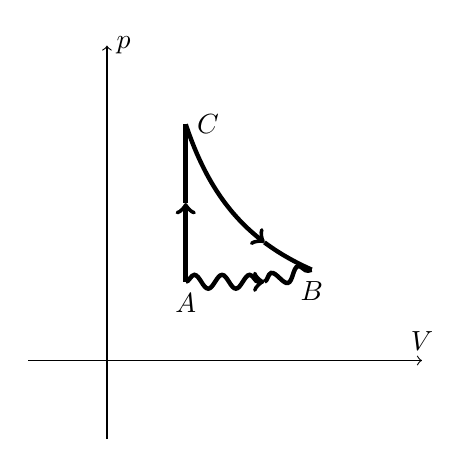
\begin{tikzpicture}[scale=2]
    \draw[->](-0.5,0)--(2,0)node[above]{$V$};
    \draw[->](0,-0.5)--(0,2)node[right]{$p$}; 
    \draw[->,ultra thick](0.5,0.5)node[below]{$A$}--(0.5,1);
    \draw[-,ultra thick](0.5,1)--(0.5,1.5)node[right]{$C$};
    \draw[->,ultra thick]plot[smooth,domain=0.5:1](\x,{0.75/(\x)});    
    \draw[-,ultra thick]plot[smooth,domain=1:1.3](\x,{0.75/(\x)});
    \draw[->,snake it,ultra thick](0.5,0.5)--(1,0.5);
    \draw[-,snake it,ultra thick](1,0.5)--(1.3,0.576)node[below]{$B$};
\end{tikzpicture}
\end{document}